%%%%%%%%%%% ******  AUTOMATED PLANNING ******* %%%%%%%%%%%%%
\section{Introduction}
\begin{center}
\textit{``Planning is an important component of rational behaviour." }\\ \cite{ghallab2004automated}
\end{center}

% \begin{center}
% \textit{``A goal without a plan is just a wish."}\\
% - Antoine de Saint-Exup\'{e}ry
% \end{center}

% Introduction/Definition
Automated planning, also known as AI planning, is an area in A.I. that studies the deliberation process of choosing and organising actions to achieve a goal. 
Humans automatically anticipate the outcome of their actions, even if they are not fully aware of it. 
Automated planning techniques are used to create information processing tools that efficiently reproduce human reasoning and behaviour. 
In particular, it can be used to model a robot's skills and strategies, when operating in diverse environments, without the need for expensive hand-coding.

The focus in automated planning lies within the development of {domain-independent} planning systems, called \textit{planners}.
These planners consist of search algorithms, which are not problem-specific, hence generate solutions to problems, no matter what the input. 
Given a set of actions, a description of the state of the world, and some goal state, the planner generates an ordered sequence of actions, which guarantees the transition from the initial state to the goal state. 
Similar to the policy derivation method mentioned in \sect{subsec:Deriving a policy}, actions are defined with \textit{preconditions}, i.e. conditions on the state of the world in order to execute the action, and \textit{effects}, i.e. changes in the state of the world after the action execution. 
%The planner produces an ordered sequence of actions, known as a \textit{plan}, which guarantees the transition from the initial state to the goal state.
There exist different types of planning:
\begin{itemize}
    \item Classical planning
    \item Optimisation: minimise or maximise a given cost function
    \item Temporal planning: actions have a certain duration, to address concurrency, synchronisation, time dependent effects
    \item Planning with preferences: prefer hard goals over soft goals
    \item Conditional planning: actions can perform observations, plan contains branches
\end{itemize}

\section{Classical planning problem}\label{subsec:Classical planning problem}
In classical planning, world dynamics are modelled as state transition systems.

\paragraph{Definition.}
A \textit{state transition system} is a triple $\Sigma = (S, A, \gamma)$ such that:
\begin{itemize}
\item $S$ is a finite set of states,
\item $A$ is a set of actions,
%\item $c : A \rightarrow \mathbb{R}^{+}$ is a cost function,
\item $\gamma : S \times A \rightarrow S$ is a state transition function.
\end{itemize}

\noindent A state transition system can be represented as a directed graph whose nodes are states of $S$, and arcs are actions of $A$. 
Applying an action $a$ to a state $s$ produces a new state $s'= \gamma(s,a)$ 
%with a cost $c(a)$
. 
$\Sigma$ is deterministic if for all states $s$ and actions $a$, the transition function $\gamma(a, s)$ produces a unique state $s'$. 
%$\Sigma$ has a unit cost if, for all $a \in A$, $c(a) = 1$. 
A \textit{plan} is any sequence of $k$ actions $\pi = <a_1,\cdots, a_k>$. The state produced by applying $\pi$ to a state $s$ is the state obtained by applying each action of $\pi$ sequentially. 
We can denote this by extending the state transition function to plans as follows:
\[\gamma(s,\pi)=\left\{
\begin{array}{ll}
   s, &\mbox{if $k=0$} \\
   \gamma(\gamma(s,a_1),<a_2,\cdots, a_k>), &\mbox{if $k>0$ and $a_1$ is applicable to $s$} \\
   \mbox{undefined}, &\mbox{otherwise}
\end{array}
\right.
\]
A state $s_n$ is reachable from a state $s_0$, if there exists a plan $\pi$ such that $s_{n} = \gamma(s_0, \pi)$.\\

%\subsubsection{Classical Planning Representations}

%Classical planning problems can be represented in three different ways, each of them being equivalent in expressive power: \cite{ghallab2004automated}

%\begin{itemize}
%\item Set-theoretic representation: each state of the world is a set of propositions, each action is a syntactic expression specifying which propositions belong to the state in order for the action to be applicable (e.g. \texttt{ontable-red, ontable-blue, on-red-blue, holding-red, holding-blue, stack-red-blue})
%\item Classical representation: states and actions are like the ones in set-theoretic representations except that first-order literals and logical connectives are used instead of propositions (e.g. \texttt{ontable(x), on(x,y), holding(x), stack(x,y)} )
%\item State-variable representation: each state is represented by a tuple of values of n state variables \{\texttt{red, blue,\dots, table, 1, 0, nil}\} (e.g. \texttt{pos(x) = table, pos(x) = y, holding = x, stack(x: block, y: block)})
%\end{itemize}

%\noindent The set-theoretic representation can take up much more space than the classical representation. The state-variable representation is less natural for logicians but useful for non-classical planning problems to handle numbers, function and time. The classical representation is the most popular choice for restricted state-transition systems \cite{ghallab2004automated}.

\noindent Logical representations are one of the most commonly used representations for classical planning problems. Each state of the world $s$ is represented by a set of logical propositions $p_i$, denoting facts of the world that are \textit{true} in the state $s$. If $p$ is not in the state $s$, it is considered to be \textit{false}.
\textit{Planning operators} change the state of the world by modifying the truth values of the propositions. An operator is defined by a set of propositions, which have to be true in a state in order to apply the changes (\textit{preconditions}), and a set of propositions, which will be true or false after the application of the action (\textit{effects}).

\paragraph{Definition.}
\noindent A \textit{planning operator} $o$ is a tuple $o = (\text{name}(o), \text{precond}(o),$ $\text{effect}(o))$, whose elements are as follows:
\begin{itemize}
\item $\text{name}(o)$ is the {\em name} of the operator,
\item $\text{precond}(o)$ is a set of literals that must be true to apply the operator $o$,
\item $\text{effect}(o)^{-}$ is a set of literals that are false after the application of the operator $o$,
\item $\text{effect}(o)^{+}$ is a set of literals that are true after the application of the operator $o$.
\end{itemize}

\paragraph{Definition.}
\noindent An \textit{action} is any ground instance of an operator. If $a$ is an action and $s$ is a state such that $\text{precond}(a)$ are true in $s$, then $a$ is {\em applicable} to $s$ and the result of applying action $a$ to state $s$ is the state $s'$:  
\[s' = \gamma(s, a) = (s - \text{effects}^{-}(a)) \cup \text{effects}^{+}(a).\]

\paragraph{Definition.}
A \textit{planning problem} in the logical representation is a quadruplet $(P, A, I, G)$ where:
\begin{itemize}
\item $P$ is a finite set of propositions,
\item $A$ is a finite set of actions,
%\item $c : A \rightarrow \mathbb{R}^{+}$ is a cost function,
\item $I \subseteq P$ is the initial state,
\item $G \subseteq P$ is the goal state.
\end{itemize}
For each $a \in A$, $\text{precond}(a)$ and $\text{effect}(a)$ are subsets of $P$ and $\text{effect}^{-}(a) \cap \text{effect}^{+}(a) = \emptyset$. The {\em state space} of a planning problem $(P, A, I, G)$ in the logical representation is a state transition system $(S, A, \gamma)$, where $S\subseteq 2^{P}$ is a subset of states defined on $P$.\\

Once this specification is provided to the planner, the planning process is a mean-ends reasoning, deciding how to achieve goals given the means of available actions. The hardness of the mean-ends planning process is high (NP-hard), as it entails non-deterministic decisions on selecting objects, committing actions on objects, sorting out actions, as well as backtracking from dead-end decisions in combinatorial search spaces.

When actions are triggered, they change the state of the world according to their effects and are not necessarily reversible. In other words, actions are not combinable in any order and have precedence constraints. For example, with the Tower of Hanoi problem, the two last actions consist of stacking the second smallest disk and then the smallest disk on the peg. Reversing the order will result in a violation of the rule that larger disks cannot be stacked onto smaller ones. Thus, plans need to be performed in the correct order to achieve the a goal.

Furthermore, the progression towards the goal is not always monotone, as actions can also have negative side effects. Consider again the Tower of Hanoi problem, where the disks need to be stacked in ascending order (smallest at the top) on the right-most peg. Our goal state is to have \textit{``disk$_{n}$ is on top of disk$_{n+1}$"} and \textit{``disk$_{n+1}$ is on the table"} for a problem with $n>0$ disks. If in the initial state the disks are stacked in ascending order on the left peg, then moving the top-most disk$_1$ to any other peg will delete the fact \textit{``disk$_1$ is on top of disk$_2$"}, and will have to be added again later to fulfill the goal.


%\subsection{STRIPS}\label{subsec:STRIPS}
%In STRIPS a closed-world assumption is used, i.e. any conditions that are not mentioned in a state are assumed to be false.


%%%%%%%%%%%%%%% *************PDDL************* %%%%%%%%%%%%%%%%%
\section{Planning Domain Definition Language (PDDL)}\label{subsec:PDDL}
Originally developed by \cite{mcdermott1998pddl} and Planning Competition Committee, the Planning Domain Definition Language (PDDL) has become the standard encoding language for classical planning tasks. It supports several syntactic features including conditional effects, specification of safety constraints and hierarchical actions composed of subactions and subgoals. PDDL expresses the ``physics'' of a domain, i.e. the available predicates, the possible actions and their effects.
The PDDL planning domain can be used to formalise the configuration of available resources together with the intended goal to eventually find a solution using PDDL planners  (\cite{huckaby2013planning}). 
%Table \ref{tab:Domain examples} shows a list of standard planning domains. 
%
%\begin{table}[h]
%\begin{center}
%\begin{tabular}{l|l|l}
%Domain & Types & Action models \\ \hline
%Blocks world & block & pick-up, put-down, stack, unstack \\
%Gripper & room, ball, gripper & pick, drop, move \\
%Tetris & L-block, S-block, I-block, T-block, O-block & pick-up, put-down, move, rotate\\
%\end{tabular}
%\end{center}
%\label{tab:Domain examples}
%\caption{Examples of possible domains with action models to be learned}
%\end{table}

\subsection{Planning domain description}\label{subsec:Planning domain description}
A PDDL planning domain consists of objects and their types, predicates describing the state of an object, and actions. Consider a planning domain that describes a standard manufacturing environment on an assembly line, with objects on the table and an arm with a gripper for manipulating them.
The head of a domain description is given as follows:
% Head of the domain description
\begin{verbatim}
(define (domain PRODUCTION)
   (:requirements :typing)
   (:types zone table - location
           metal wood - product)
   (:constants right - gripper)
   (:predicates (at-gripper ?g - gripper ?l - location)
                (at ?p - product ?l - location)
                (free ?g - gripper)
                (empty ?l - location)
                (carry ?p - product ?g - gripper))
\end{verbatim}
\noindent
A domain description always starts with the declaration of its name, preceded by the keyword \texttt{domain}. Then, the requirements of the domain are defined, identified by the keyword \texttt{:requirements}. The requirements allow to characterise the expressiveness of the domain description. For instance, in the domain description above, the requirements specify that action descriptions can use typed terms. In other cases, preconditions with equality terms, and effects, with conditional and universal quantifier terms, can also be specified. 

All domains define a few primitive types from which it is possible to derive all the types necessary for the domain description. In the \texttt{PRODUCTION} domain example, the type \texttt{metal} and \texttt{wood} are derived from the type \texttt{product}. The type descriptions are identified by the keyword \texttt{:types}. The keyword \texttt{:constants} defines the values that remain unchanged and that can be referenced directly.

The predicates, identified by the keyword \texttt{:predicates}, specify what facts (about objects in the world) can be used in the preconditions and effects of the operators. Predicates can have arguments of specified types. An argument term starts with a question mark ``\texttt{?}". For instance, \texttt{(at ?p - product ?l - location)} expresses that a variable \texttt{?p}, whose type is \texttt{product}, is located at location \texttt{?l}.

The above planning domain is comprised of the following predicates, which can be seen as logical symbols:

\begin{table}[h]
\begin{center}
\begin{tabular}{l|l}
Predicate & Description\\ \hline
\texttt{at-gripper ?g - gripper ?l - location} & The gripper \texttt{?g} is at position \texttt{?l}.\\
\texttt{at ?p - product ?l - location} & The product \texttt{?p} is at location \texttt{?l}.\\
\texttt{free ?g - gripper} & The gripper \texttt{?g} is free.\\
\texttt{carry ?p - product ?g - gripper} & The gripper \texttt{?g} is holding product \texttt{?p}.\\
\texttt{empty ?l - location} & The location \texttt{?l} is empty.\\
\end{tabular}
\end{center}
\label{tab:predicates}
\caption{Predicates for the \texttt{PRODUCTION} domain}
\end{table}%


In a domain description, operators, i.e. first-order actions, specify the different ways to perform changes to the world state. 
Consider a simple action model \texttt{pick} for a pick-up action, which consists of grasping an object with the gripper and results in lifting it off the table.
\begin{verbatim}
(:action pick
    :parameters (?p - product ?l - location ?g - gripper)
    :precondition  (and  (at ?p ?l) (at-gripper ?g ?l) 
                         (free ?g) not(empty ?l))
    :effect (and (carry ?p ?g)
                 (empty ?l)
                 (not (at ?p ?l)) 
                 (not (free ?g))))
\end{verbatim}

This action means that a product \texttt{?p} can be picked up, if both the gripper \texttt{?g} and the product are at the location \texttt{?l} and the gripper is free (preconditions). After the \texttt{pick} action execution, the effects express that the gripper \texttt{?g} is currently carrying the product \texttt{?p}, that it is not free anymore and that the product is no longer placed at location \texttt{?l}.

In general, an action model consists of the following:
\begin{itemize}
\item \texttt{:parameters} -- variables on which the action model operates,
\item \texttt{:precondition} -- conditions that must be satisfied before the action can be executed; if none are specified, the action is always executable,
\item \texttt{:effect} -- changes in the world state imposed by the action.
\end{itemize}
The \texttt{PRODUCTION} domain consists of the three actions: \texttt{pick, drop} and \texttt{move}. Similar to the \texttt{pick} action, \texttt{drop} can be specified as follows:
\begin{verbatim}
   (:action drop
       :parameters  (?p - product ?l - location ?g - gripper)
       :precondition  (and  (carry ?p ?g) (at-gripper ?g ?l) (empty ?l))
       :effect (and (at ?p ?l)
                    not(empty ?l)
                    (free ?g))))
\end{verbatim}
In this action, product \texttt{?p} is dropped at a location \texttt{?l}. The preconditions assert that product \texttt{?p} has to be carried by the gripper \texttt{?g} and that the gripper \texttt{?g} is at the location \texttt{?l}, which is empty.  The effects mean that after the action execution, the product \texttt{?p} occupies location \texttt{?l} and that the gripper \texttt{?g} is free. \\
Consider the last action in our domain:
\begin{verbatim}
   (:action move
       :parameters  (?g - gripper ?from ?to - location)
       :precondition (at-gripper ?g ?from)
       :effect (and  (at-gripper ?g ?to)
                     (not (at-gripper ?g ?from))))
\end{verbatim}
This specifies that the gripper \texttt{?g} moves from a starting position \texttt{?from} to a target position \texttt{?to}, if the gripper is initially at starting position \texttt{?from}. The predicates \texttt{(at-gripper ?g ?to)} and \texttt{(not (at-gripper ?g ?from))} in the effect description ensure that the gripper is not at two positions at the same time.
%\begin{itemize}
%\item Example state of the art: (example action sequence)
 % \item{   Manufacturing tasks require extra overhead to {reprogram the robot} when the process of the task changes.  }
  %\item{   A key issue in PbD is to {design a generic system} to teach skills that can be used in different situations.  }
  %\item{   Current implementations include an {intermediate manual step to construct action sequences} to arrive to a goal state.  }
%  \end{itemize}

\subsection{Planning Problem Description}\label{subsec:PPDescription}
In manufacturing domains, there exist installation procedures for various devices that need to be strictly followed. It can happen that assembly parts need to be moved around in the work place. Consider a planning problem for the \texttt{PRODUCTION} domain defined as:
\begin{verbatim}
(define (problem PERMUTATION)
   (:domain PRODUCTION)
   (:requirements :typing)
   (:objects zoneA zoneB - zone
             table - table
             engine - metal
             hood - metal)
   (:init (at-gripper zoneA)
          (free right)
          (at engine zoneB)
          (at hood zoneA))
   (:goal (at engine zoneA)
          (at hood zoneB)))
\end{verbatim}

The \texttt{PERMUTATION} planning problem starts by listing all objects of the world and their initial state. This world is composed of three locations, \texttt{zoneA}, \texttt{zoneB} and the \texttt{table}, and two installation devices, \texttt{engine} and \texttt{hood}, which are both of type \texttt{metal}. The engine needs to be installed before the hood, therefore the engine needs to be placed in \texttt{zoneA} and the hood needs to be in \texttt{zoneB}. As devices on assembly lines arrive arbitrarily, depending on the completion time of the previous task, it is possible that they arrive in the reversed order. Given only one gripper, the goal is to find a plan to move \texttt{engine} from \texttt{zoneB} to \texttt{zoneA} and \texttt{hood} from \texttt{zoneA} to \texttt{zoneB}. 

Another planning problem in this domain could include multiple parts on the assembly line, which need to be manipulated in a given order. 
As we can define an infinite number of objects in our planning domain, there exist an infinite number of planning problems that can be defined and solved. PDDL provides a means to model any real-world environment in the form of a planning domain. 

\begin{figure}[!h]
	\centering
	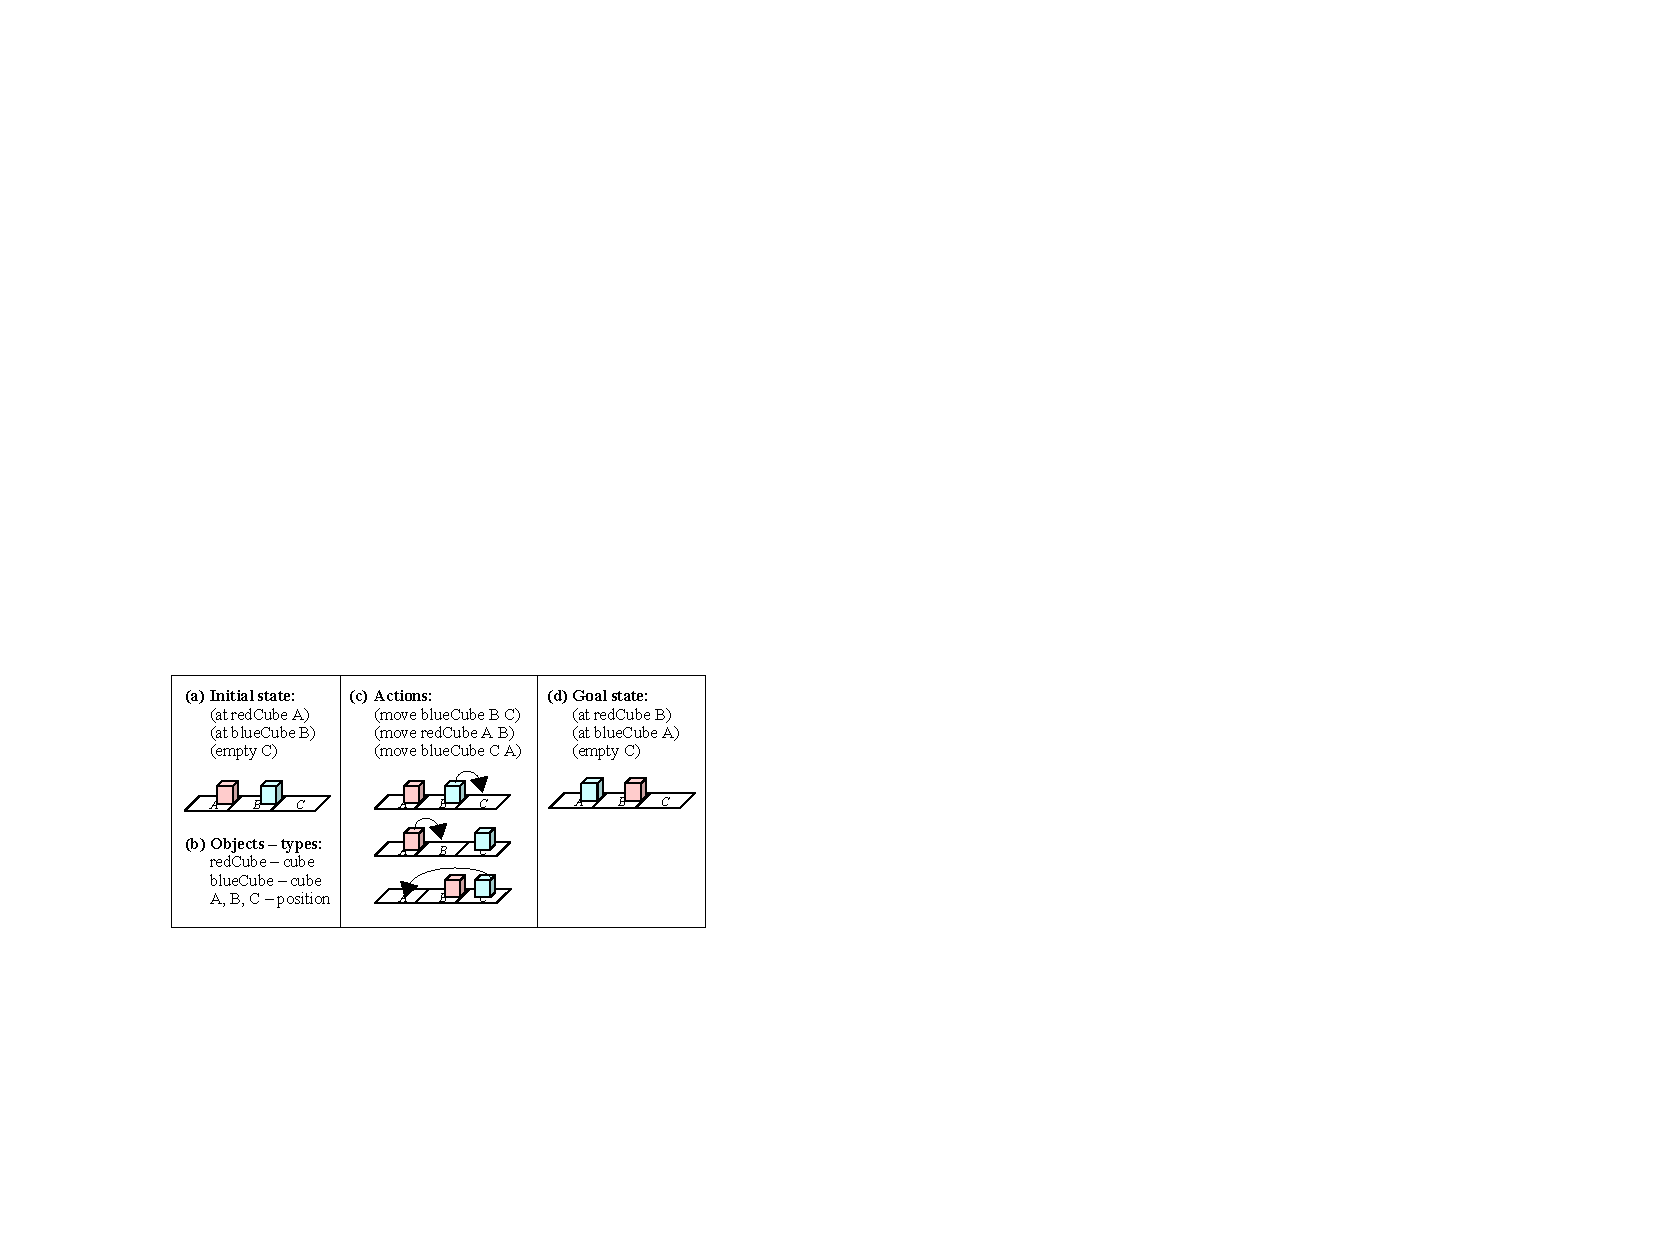
\includegraphics[width=0.48\linewidth]{figures/planning-permutation}
	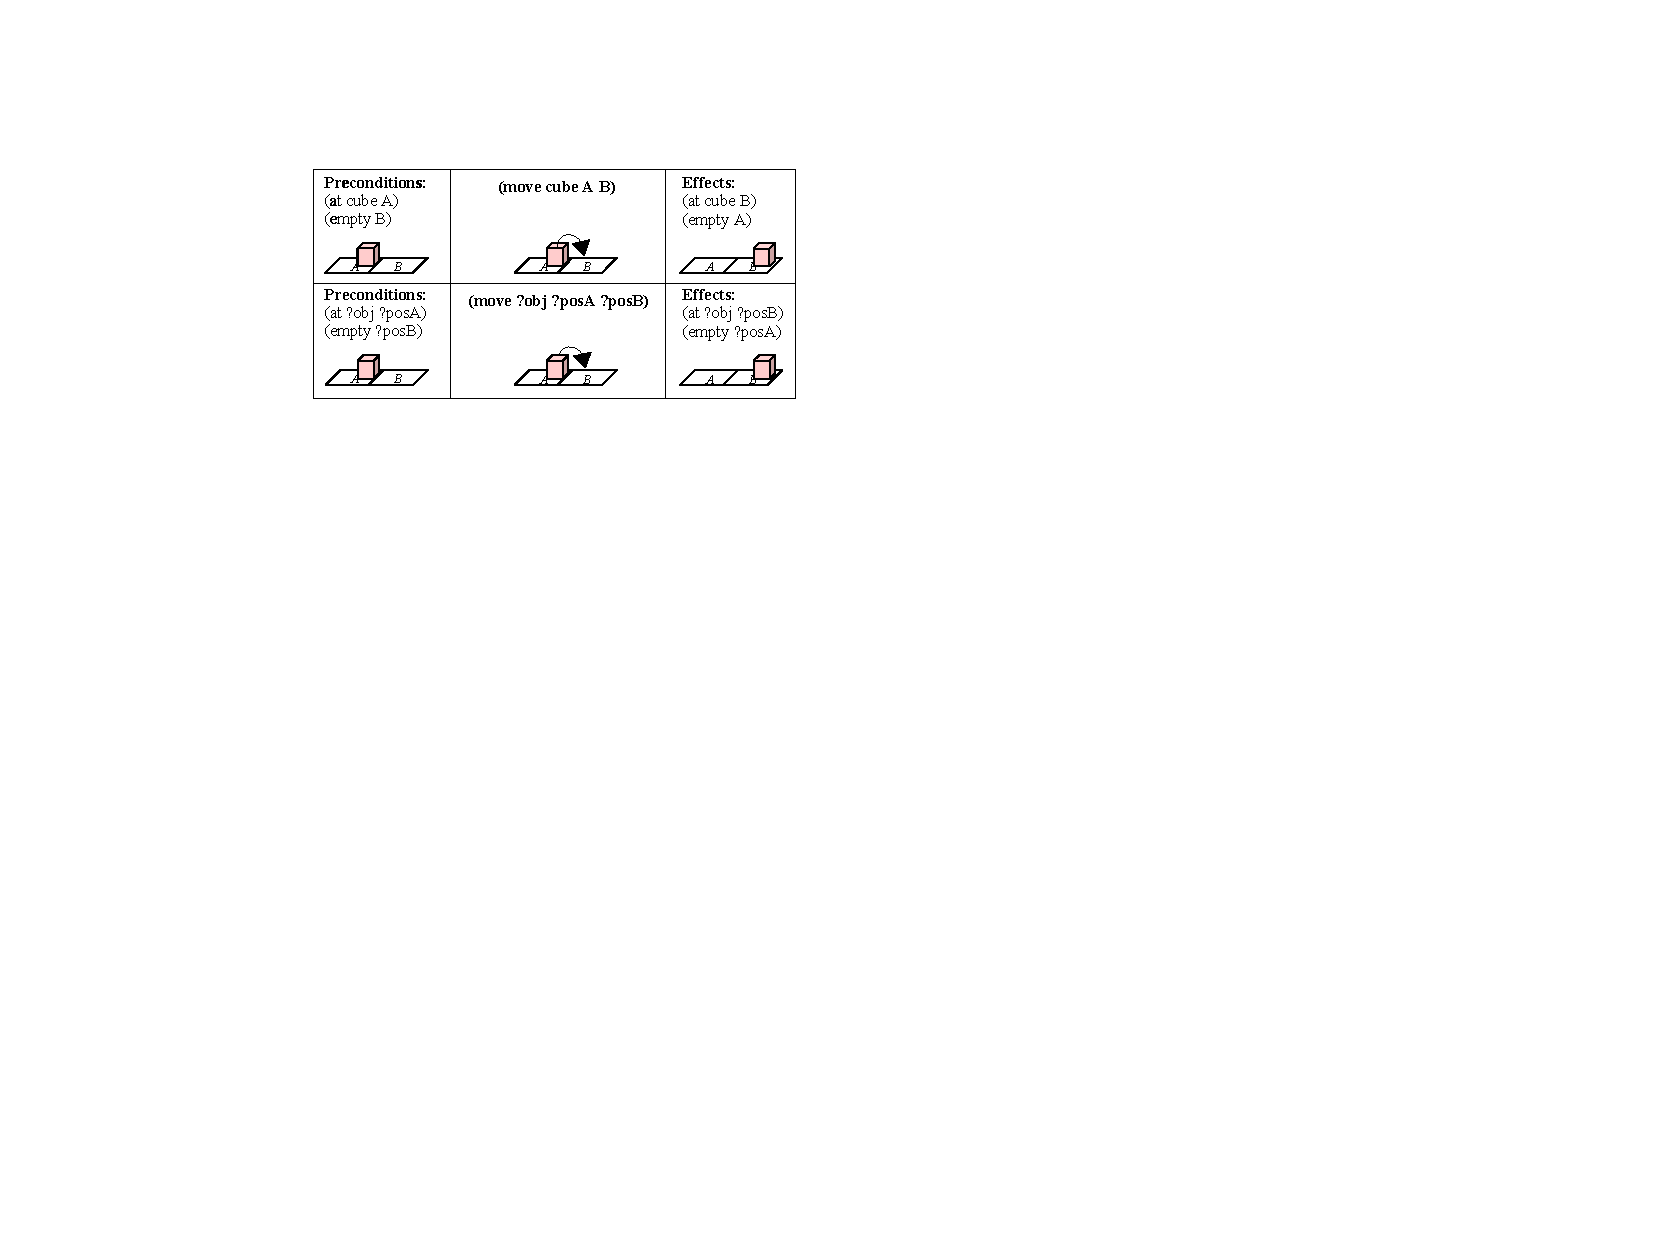
\includegraphics[width=0.48\linewidth]{figures/schema-logic}
	\caption{Definition of a planning problem: Left: (a) properties describing the initial world state (b) object names and their types (c) instantiated actions (d) properties describing the goal state. Right: Action model representation of a move action in terms of preconditions and effects: demonstrated action model for a cube (top), and generalised action model for any object, variables are prefixed with `?' (bottom).}
	\label{fig:action}
\end{figure}
\subsection{Relation to Present Work}
In general, the majority of tasks can be completed using the simple actions pick, move and drop. For our framework, we considered planning problems, such as the Tower of Hanoi problem (\cite{douglas1985metamagical}) or a real-life game of Tetris (\cite{tetris}), which use these actions. Since we focus on applications in cobotic environments, we wanted to choose a planning problem that occurs in real-world applications. Therefore, we chose to evaluate the usability of our framework using the \texttt{PRODUCTION} planning domain, addressing the \texttt{PERMUTATION} planning problem. It is then easy for the user to extrapolate from this simple example to any complex task.

\fig{fig:planning-permutation} illustrates an example of the permutation planning problem. Given a description of the world state, i.e. objects, types, properties (\fig{fig:planning-permutation}a,b), a set of possible atomic actions, and a goal state (\fig{fig:planning-permutation}d), the planner should generate the correct sequence of actions (\fig{fig:planning-permutation}c), which guarantees the transition from the initial world state to the goal state. Predicates are used to describe actions and object properties, such as \textit{``red cube is at position A"}: they can be \textit{instantiated} \texttt{(at redCube A)} or \textit{generalised} \texttt{(at ?cube ?posA)}, such that variables are prefixed with `?'.

To allow a correct transition between different states of the world, actions are defined in terms of {preconditions} and {effects} (\fig{fig:action}). For a move action \texttt{(move cube A B)}, preconditions are the states required to perform the action  \texttt{(at cube A)}, and effects are the states obtained after the action \texttt{(at cube B)}. Classical planning algorithms use the Planning Domain Definition Language (PDDL) \cite{ghallab2004automated} as their standard encoding language, which extends the STRIPS \cite{fikes1971strips} formalism with greater expressivity, such as type structures (\fig{fig:planning-permutation}b). 

%Our proposed framework targets these domains and aims at solving related planning problems. It will allow the user to create action models and link the planning problem with the actual physical action executed by the robot.

% To Do: Discuss related work in terms of subjects that are addressed by Robot Programming by Demonstration in Cobotic Environments


\subsection{PDDL evolution and extensions}\label{subsec:PDDL evolution}

Ever since the first version of \textsc{Pddl} 1.2 (\cite{mcdermott1998pddl})was introduced as the official language of the 1st \textsc{Ipc} (International Planning Competition), there have been several new versions and extensions. 
Succeeding versions that allow the representation of real-world problems had a particular influence on the adaptation of planners with robots in cobotic environments. In 2002, \textsc{Pddl} 2.1 introduced functions to express numerical objects, durative actions and plan-metrics for assessing plan quality. 
An extension called \textsc{Mapl} (Multi-Agent Planning Language), introduced finite domain state-variables, actions with duration determined in runtime, and explicit plan synchronisation obtained through speech acts and communications among agents. 
The newly introduced functionalities are particularly useful for cobotic environments to incorporate actions of varying durations into the planning system, or to allow multi-agent planning for several robots to collaborate in the same environment.
In the following years \textsc{Ppddl} (Probabilistic \textsc{Pddl})(\cite{younes:04a}) was proposed, extending \textsc{Pddl} 2.1 with probabilistic effects and introducing partial observability. This extension opened up the possibility to integrate statistical models into the planning system and improved the robot's learning capabilities and performance in uncertain situations. Cobots can benefit from this as they are often faced with uncertain situations, when working with different human operators, who have varying behaviours.

\subsection{Planners}\label{subsec:Planners}
Automated planners have found its increasing application in various areas from aeronautics and space to agricultural and industrial domains (\cite{aarup1992optimum}). We conclude this section by introducing the most significant planners for classical planning, that have been implemented to date. The simplest planners are state-space planners, which rely on search algorithms in which the search space is a subset of the state space. Each node corresponds to a state of the world, each arc represents a state transition, i.e. an action, and a plan is a path from the initial state to a goal state in the search space (\cite{ghallab2004automated}). An extended version of the planner is the Heuristics Search Planner (\cite{bonet:01}), which includes several basic search algorithms like best-first search, breadth-first-search, A* and iterative deepening search. The Fast-Forward planning system (\cite{hoffmann:11}) is based on the HSP, but managed to outperform it, due to modifications aimed to avoid getting trapped in local minima (\cite{hoffmann2000heuristic}): It includes a variation of the hill-climbing search, called the \textit{enforced hill climbing}, and a heuristic called \textit{helpful actions}. Finally, Fast Downward (\cite{helmert:06a}) is a state-space planner based on a finite domain representation, with a greedy best-first search as its main search procedure. 

Another category are planning-graph planners, which carry out the search by encoding the search space in a structure called the \textit{planning graph}. It considers the union of sets of propositions of several states rather than individual states. The first planner being the Graphplan (\cite{blum:97}), which uses a backward search and replaces the goal with preconditions. Other planners include SATPlan (\cite{kautz:06,kautz:99}) and the GP-CSP (\cite{do:01}).